\documentclass[10pt]{beamer}
\usetheme[progressbar=frametitle]{metropolis}

\usepackage{appendixnumberbeamer}
\usepackage{booktabs}
\usepackage[scale=2]{ccicons}
\usepackage{pgfplots}
\usepgfplotslibrary{dateplot}
\usepackage{xspace}
\usepackage{amsmath}
\usepackage{amssymb}
\usepackage{subfig}
\usepackage{graphicx}
\usepackage{caption}
\usepackage{pdfpages}

\graphicspath{ {./images/} }

\newcommand{\themename}{\textbf{\textsc{metropolis}}\xspace}

\title{Brief discussion on 3D pose estimation\\
based on article: "3D pose estimation of visual markers"}
\subtitle{Author: Antonio Badal Regàs}
% \date{\today}
\date{}
\author{Aziel Martins de Freitas Júnior}
\institute{SENAI CIMATEC}
% \titlegraphic{\hfill\includegraphics[height=1.5cm]{logo.pdf}}

\begin{document}

\maketitle

%----------------------SLIDE 01----------------------%

\begin{frame}{Contents}

  \setbeamertemplate{section in toc}[sections numbered]
  \tableofcontents%[hideallsubsections]

\end{frame}

\section[Introduction]{Introduction}

%----------------------SLIDE 02----------------------%

\begin{frame}[fragile]{Motivation}

  Study arised from the need to understand, analyze and improve a computer vision software based on the \emph{ARToolKitPlus} software library.

\end{frame}

%----------------------SLIDE 03----------------------%

\begin{frame}[fragile]{ARToolKit}
  \begin{columns}
    % Left column
    \column{0.5\textwidth}
    \begin{itemize}
      \item First article published in 1999;
      \item Intended for augmented reality in collaborative office work;
      \item One user would wear a HMD (\emph{head mounted display}) to provide others augmented reality visuals.
    \end{itemize}
    % Right column
    \column{0.5\textwidth}
      \begin{figure}
        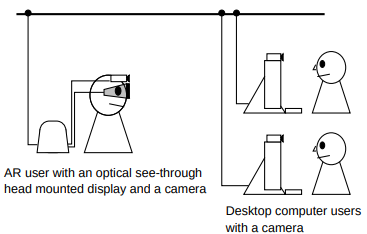
\includegraphics[scale=0.35]{1999-sysoverview}
        \caption{Intended usage.}
      \end{figure}
      \begin{figure}
        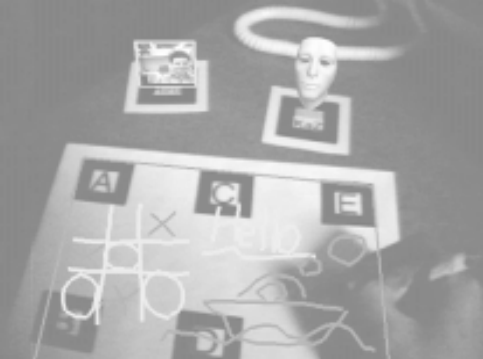
\includegraphics[scale=0.25]{1999-virtboard}
        \caption{HMD image.}
      \end{figure}
  \end{columns}


\end{frame}

%----------------------SLIDE 04----------------------%

\begin{frame}[fragile]{MBV: Marker-based vision systems}

  \begin{itemize}
    \item Dependent on \textbf{fiducial markers};
    \item \emph{ARtag} are commonly used;
    \item Tag family for this study was not specified;
    \item \emph{ARToolKitPlus} system was used because of it's accurate readings.
  \end{itemize}

\end{frame}

%----------------------SLIDE 05----------------------%

\begin{frame}[fragile]{Square and circular ARtags}

  Cons: square AR tags have the disadvantages of occlusion and minimum size detection when in comparison.

  Pros: square have low false negative and very low confusion rate when used in groups.

  \begin{figure}
    \centering
    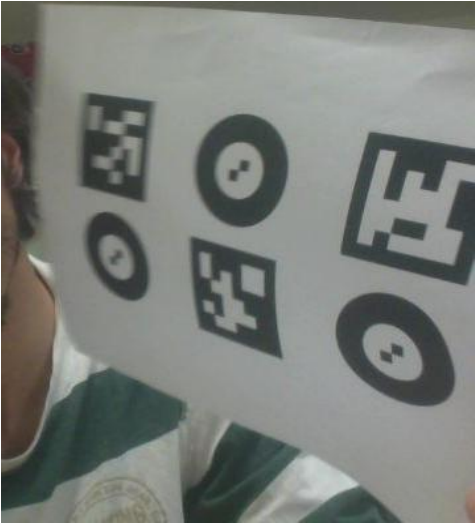
\includegraphics[scale=0.1]{tags}
    \caption{Examples of tags used by the author. Only the square ones were used in the article.}
  \end{figure}

\end{frame}

%----------------------SLIDE 06----------------------%

\begin{frame}[fragile]{Concept - space transformation}

  The act of fitting a space image information into a plane;

  Typical of pinhole cameras;

  Two space transformations \textbf{may happen} to the acquired image: a rotation and a translation.

  \begin{figure}
    \centering
    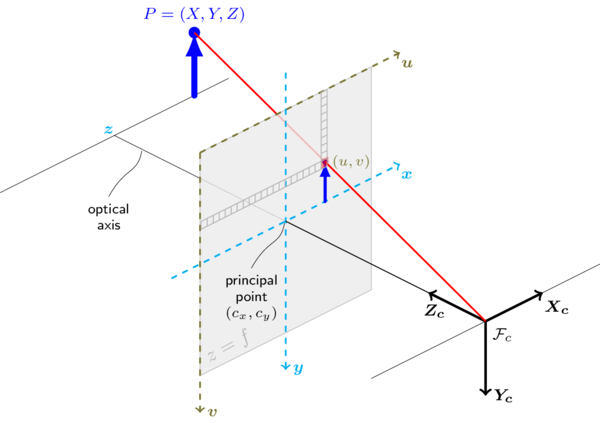
\includegraphics[scale=0.3]{space_transf}
    \caption{Projection example.}
  \end{figure}

\end{frame}

%----------------------SLIDE 07----------------------%

\begin{frame}[fragile]{Core concept - space transformation}

  Transformation represented by:
  \begin{align*}
    v_i=K\times\mathcal{R}\times p_i+\mathcal{T}
  \end{align*}
  $v_i$ is each projected $p_i$ point of the real world object. $K$ depends on the camera lenses.
  The world object \textbf{may have suffered} a rotation $\mathcal{R}$ and a translation $\mathcal{T}$:
  \begin{align}
    s \cdot
    \begin{pmatrix}
      u \\ v \\ 1
    \end{pmatrix}
    =
    K_{3 \times 3} \times
    \begin{pmatrix}
    r_{11} & r_{12} & r_{13} \\
    r_{21} & r_{22} & r_{23} \\
    r_{31} & r_{32} & r_{33} \\
    \end{pmatrix}
    \times
    \begin{pmatrix}
      x \\ y \\ z
    \end{pmatrix}
    +
    \begin{pmatrix}
      T_x \\ T_y \\ T_z
    \end{pmatrix}
  \end{align}

  Goal - obtain $\mathcal{R}$ and $\mathcal{T}$ with iterative error minimization via Newton-Raphson's method.
\end{frame}
%----------------------SLIDE 08----------------------%
\begin{frame}[fragile]{Goals}
  \begin{itemize}
    \item Obtain applicable information on marker identification;
    \item Examine software problems and improve item;
    \item Test, criticize and improve.
  \end{itemize}

\end{frame}

\begin{frame}[fragile]{Concept map}
  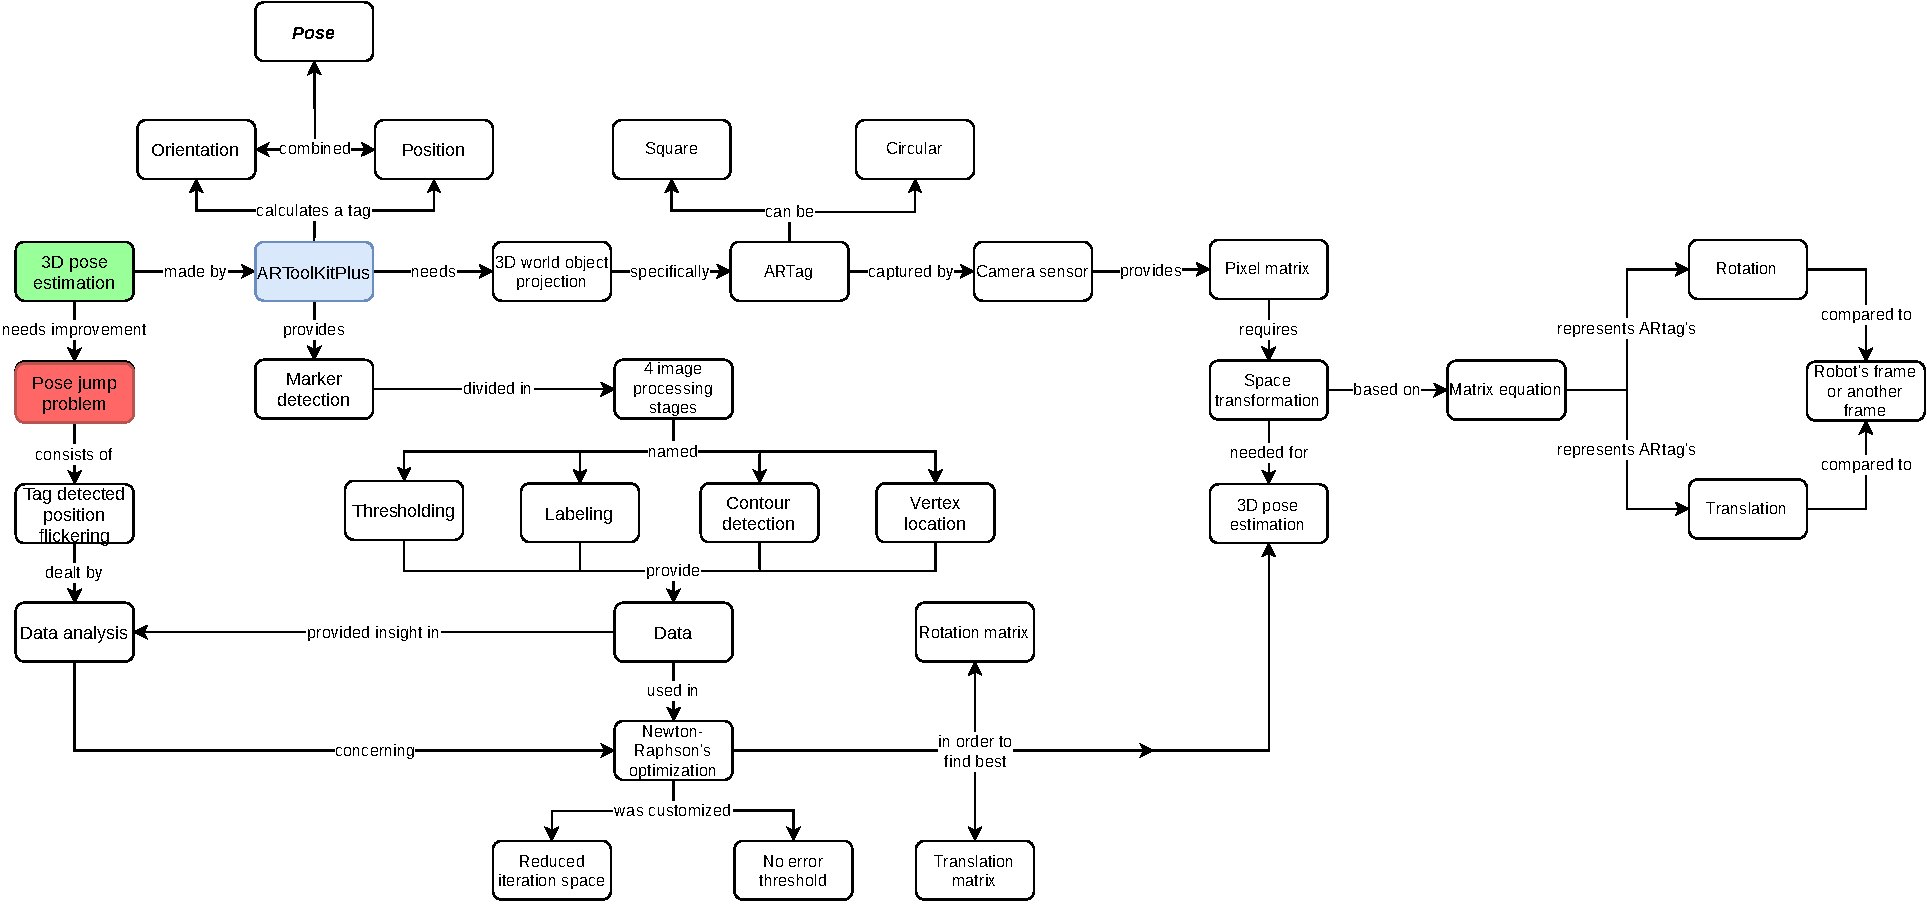
\includegraphics[scale=0.35]{./concept_map/concept_map.pdf}
\end{frame}

%----------------------SLIDE 09----------------------%

\section{Problem presentation}

%----------------------SLIDE 10----------------------%

\begin{frame}[fragile]{Pose jump}

  \begin{columns}
    % Left column
    \column{0.5\textwidth}
      What is pose jump?
      \begin{itemize}
        \item Tag kept in place while RViz shows tag frame in two different places and orientations;
      \end{itemize}
    % Right column
    \column{0.5\textwidth}
      \begin{figure}
        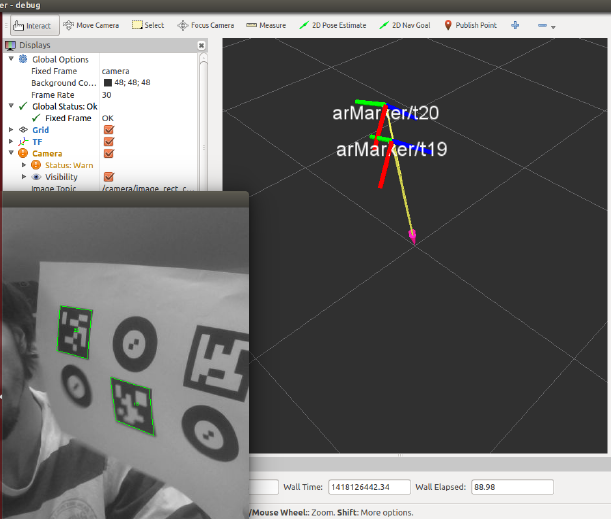
\includegraphics[scale=0.15]{pj01}
        \caption{First tag placement.}
      \end{figure}
      \begin{figure}
        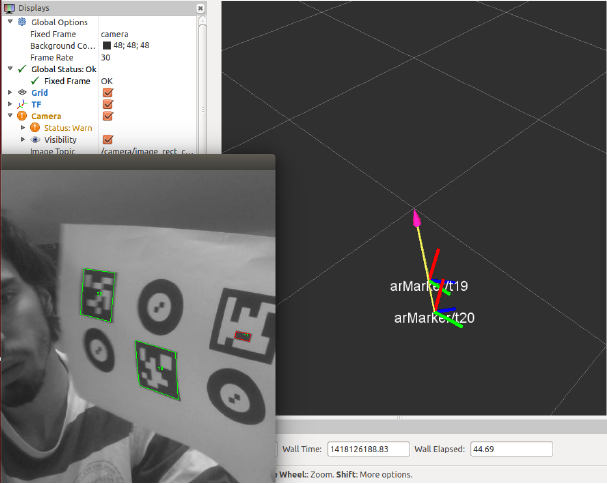
\includegraphics[scale=0.15]{pj02}
        \caption{Second tag placement.}
      \end{figure}
  \end{columns}

\end{frame}

%----------------------SLIDE 11----------------------%

\begin{frame}[fragile]{Pose jump table}

  \begin{figure}
    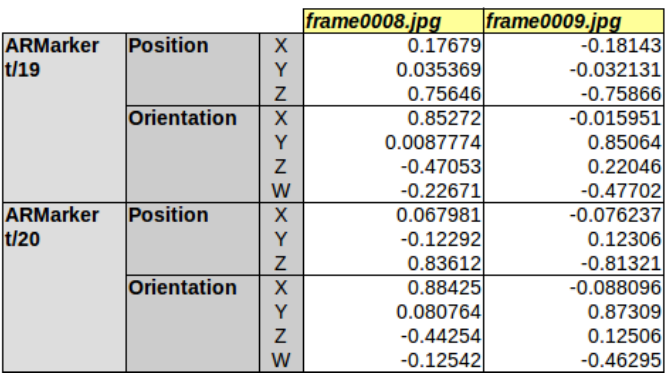
\includegraphics[scale=0.4]{pj_table}
    \caption{Different placement in two different moments.}
  \end{figure}

\end{frame}

%----------------------SLIDE 12----------------------%

\begin{frame}[fragile]{Placement over time}

\vspace{0.5 cm}
  \begin{figure}
    \centering
    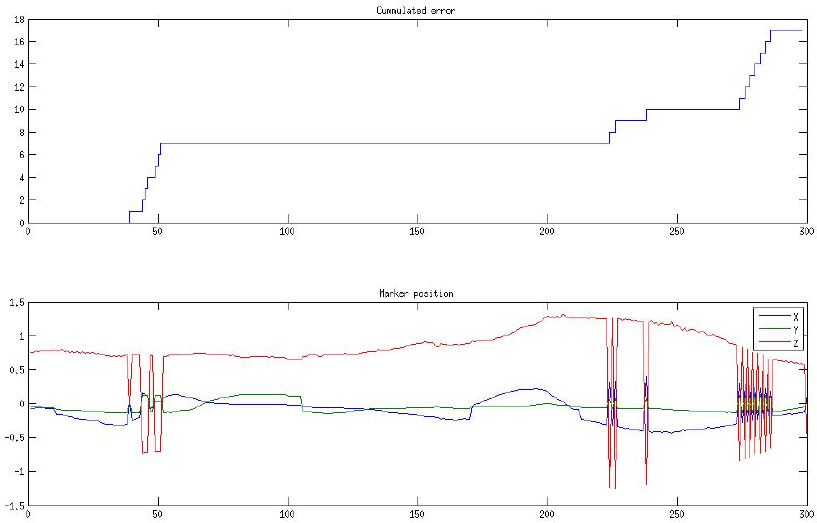
\includegraphics[scale=0.35]{300frames01}
    \caption{Frame placement along 300 frames.}
  \end{figure}

\end{frame}

%----------------------SLIDE 13----------------------%

\begin{frame}[fragile]{Symmetry hint}
  Clearer sign that symmetry is part of the problem.
    \begin{figure}
      \centering
      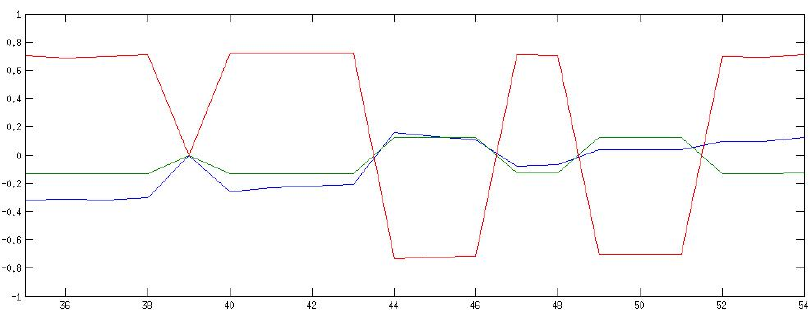
\includegraphics[scale=0.35]{zoomat50}
      \caption{Abrupt changes of Z are origin symmetric.}
    \end{figure}

  \end{frame}

%----------------------SLIDE 14----------------------%

\section{Software operation \\ and possible issues}

%----------------------SLIDE 15----------------------%

\begin{frame}[fragile]{Operation steps}
  \begin{columns}
    \column{0.3\textwidth}
      \begin{itemize}
        \item Camera calibration;
        \item Marker detection;
        \item Pose calculation;
        \item Pose visualization.
      \end{itemize}
    \column{0.7\textwidth}
      \begin{figure}
        \centering
        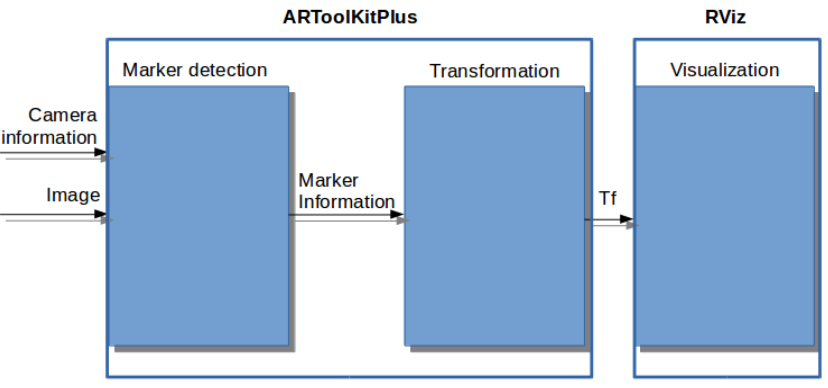
\includegraphics[scale=0.25]{softwarediagram}
        \caption{Steps to the output.}
      \end{figure}
  \end{columns}
\end{frame}

%----------------------SLIDE 16----------------------%

\begin{frame}[fragile]{Core process: marker detection}
  \begin{itemize}
    \item Thresholding;
    \item Labeling;
    \item Contour detection;
    \item Vertex localization;
    \item Tag identification and localization.
  \end{itemize}
\end{frame}

%----------------------SLIDE 17----------------------%

\begin{frame}[fragile]{Thresholding}
  Establish intensity limits to tag readability;

  Each pixel is evaluated:
    \begin{equation*}
      r+g+b<\text{threshold}\times 3
    \end{equation*}
  Saves processing efforts on Labeling step.
\end{frame}

%----------------------SLIDE 18----------------------%

\begin{frame}[fragile]{Labeling - image segmentation}
  Evaluation of image continuity by pixel surroundings analysis.
  \begin{figure}
    \centering
    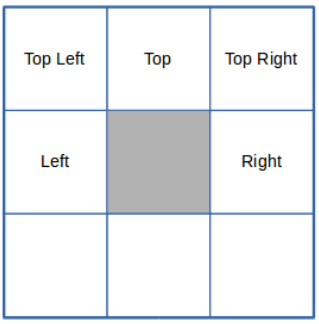
\includegraphics[scale=0.25]{labeling}
    \caption{Matrix for labeling process.}
  \end{figure}
  A pixel shares it's neighbors label whenever they are continuous.
\end{frame}

%----------------------SLIDE 19----------------------%

\begin{frame}[fragile]{Contour detection}
  Intuitive contour discerning method.
  \begin{figure}
    \centering
    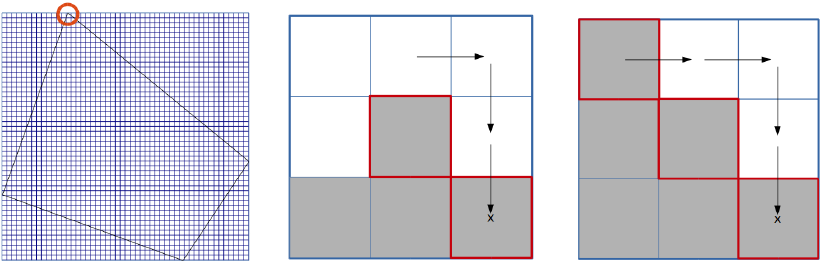
\includegraphics[scale=0.35]{contour}
    \caption{Contour detection process.}
  \end{figure}
\end{frame}

%----------------------SLIDE 20----------------------%

\begin{frame}[fragile]{Vertex location}
  \begin{columns}
    \column{0.4\textwidth}
      Most distant point pair is located;\\
      Line is traced between them;\\
      Other vertices are found.
    \column{0.6\textwidth}
      \begin{figure}
        \centering
        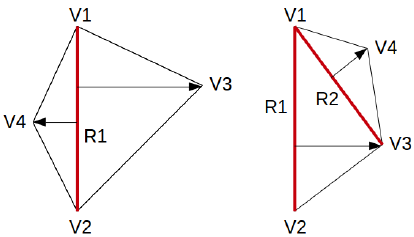
\includegraphics[scale=0.35]{vertex}
        \caption{Vertex location.}
      \end{figure}
  \end{columns}
\end{frame}

%----------------------SLIDE 21----------------------%

\begin{frame}[fragile]{Why all this?}
  \begin{columns}
    \column{0.4\textwidth}
      The computations made before provide the inputs;\\
      If evaluation results in a valid tag, there will be outputs;\\
      The outputs will then provide for the pose estimation.
    \column{0.6\textwidth}
      \begin{figure}
        \centering
        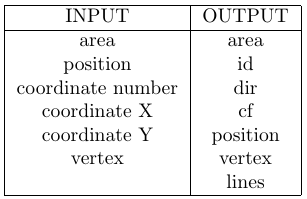
\includegraphics[scale=0.35]{partial-table}
        \caption{Partial table for evaluated tag.}
      \end{figure}
  \end{columns}
\end{frame}

%----------------------SLIDE 22----------------------%

\begin{frame}[fragile]{Iterative pose transformation}
  Newton-Raphson iterative method for minima is applied;\\
  Targets: $\mathcal{R}$ and $\mathcal{T}$ of each vertex.
  \begin{itemize}
    \item Initial guess for $\mathcal{R}$ and $\mathcal{T}$;
    \item Guess is applied to the 3D-2D transformation equation;
    \item The residuals $x$ and $y$ for each vertex are calculated;
    \item Each pair $x_i, y_i$ of residue for each vertex is used to compute the corrections to translation and rotation;
    \item Iteration ends when residues are small enough.
  \end{itemize}
\end{frame}

%----------------------SLIDE 23----------------------%

\begin{frame}[fragile]{The culprit}
  \begin{columns}
    \column{0.5\textwidth}
      The author excludes camera calibration, marker detection and quaternion transformation as reasons for the pose jump based on the low \textbf{\% error} values seen in the table.\\
      That leaves the iteration as the reason.
    \column{0.5\textwidth}
    \vspace{-0.5 cm}
      \begin{figure}
        \centering
        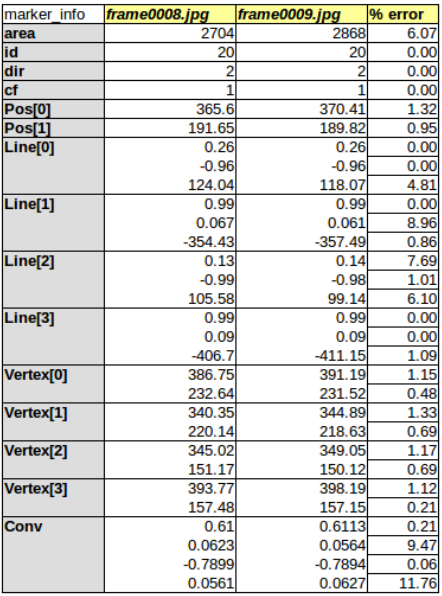
\includegraphics[scale=0.35]{table-extended.png}
        \caption{Pose jump error accounted.}
      \end{figure}
  \end{columns}
\end{frame}

%----------------------SLIDE 24----------------------%

\section{Conclusion - proposed solution}

%----------------------SLIDE 25----------------------%

\begin{frame}[fragile]{Actions taken}
  The iteration error threshold should be turned off so the optimization algorithm does one more attempt at getting small error values;\\
  Iteration algorithm attempts 30 sweeps of 15$^{\circ}$;\\
  Reduction to sweeps of 5$^{\circ}$.\\
  \begin{figure}
    \centering
    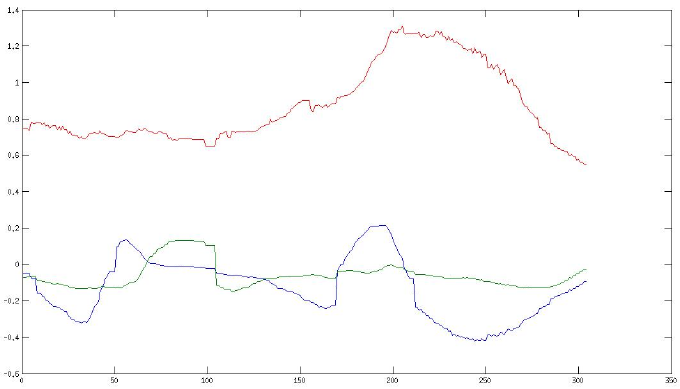
\includegraphics[scale=0.35]{no-jumps.png}
    \caption{No position jumps registered.}
  \end{figure}
\end{frame}

\end{document}
